\titleformat{\chapter}[display]
{\normalfont\huge\bfseries}{Capítulo \thechapter}{0.5em}{\huge}
\titlespacing*{\chapter}{0pt}{-1.25cm}{25pt}
\chapter{Introducción}
\section{¿Qué es APRS?}

El APRS o Sistema Automático de Reporte de Paquetes (APRS, por sus siglas en inglés: Automatic Packet Reporting System) es un sistema de comunicaciones digitales en tiempo real que permite el intercambio de información entre estaciones de radioaficionados.

De manera general, APRS se utiliza para el rastreo de vehículos, la transmisión de mensajes de texto, la diseminación de información meteorológica y la comunicación en situaciones de emergencia aunque debido a la flexibilidad del protocolo puede ser usado en cualquier otra situación.

\begin{figure}[h!]
	\centering
	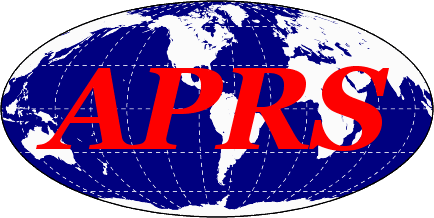
\includegraphics[width=0.2\textwidth]{./Chapter_1/APRS_logo.png}
	\caption{Logo de APRS.}
	\label{fig:aprs-logo}
\end{figure}

\section{Características Principales de APRS}

APRS posee varias características que lo hacen útil y versátil en el ámbito de la comunicación de radioaficionados, entre las cuales se encuentran las siguientes:
\begin{itemize}
	\item \textbf{Frecuencia de Operación:} APRS opera en la banda de VHF, específicamente en la frecuencia de 144.80 MHz en Europa, aunque en otras regiones del mundo se utilizan frecuencias diferentes tal como se muestra en la figura \Cref{fig:freq-map}.
	\item \textbf{Modo de Transmisión:} APRS utiliza como modo de transmisión paquetes individuales que han de seguir un formato establecido, esto facilita enormemente la adopción e integración de esta tecnología.
	\item \textbf{Actualización de Datos en APRS:} En el sistema APRS, un paquete de información se transmite múltiples veces, disminuyendo gradualmente la frecuencia de envio de estas transmisiones a medida que el tiempo avanza. Este método tiene como objetivo maximizar la tasa de recepción de los paquetes.
\end{itemize}

\begin{figure}
	\centering
	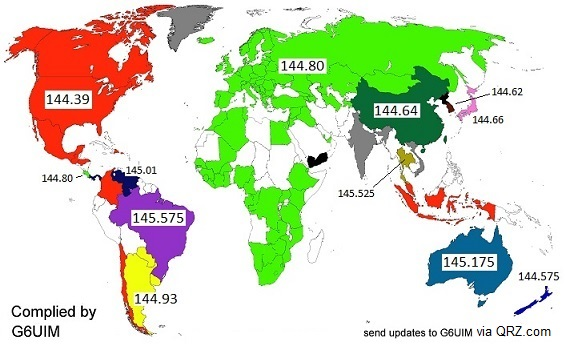
\includegraphics[width=0.5\textwidth]{./Chapter_1/mapa_frecuencias_aprs.jpg}
	\caption{Mapa de frecuencias APRS en el mundo.}
	\label{fig:freq-map}
\end{figure}


\section{Usos Principales de APRS}

\begin{itemize}
	\item \textbf{Reportes GPS:} APRS permite a los usuarios enviar su ubicación geográfica en forma de coordenadas, obtenida a través de sistemas GPS, lo que facilita el seguimiento de vehículos o personas en tiempo real.

	\item \textbf{Datos Meteorológicos:} Las estaciones meteorológicas suelen utilizar mensajes APRS para reportar diferentes datos como temperatura, humedad o presión barométrica, incluyendo información actualizada y útil para diversas aplicaciones.

	\item \textbf{Integración con Internet:} Mediante el sistema APRS-IS, los mensajes APRS son accesibles por internet a través de distintos nodos, ampliando el alcance y la extensión de este sistema.

	\item \textbf{Uso en Emergencias:} En situaciones de emergencia, APRS es una herramienta vital para la comunicación de broadcast y el seguimiento de recursos y personal.
\end{itemize}

\section{Historia y Desarrollo de APRS}

El sistema APRS nació en la decada de los 80 de la mano de Bob Bruninga, un ingeniero que trabajaba como en la Academia Naval de los Estados Unidos. Bruninga creó la primera implementación de APRS en un ordenador Apple II en 1982 con el objetivo de mapear informes de posición de la Marina en alta frecuencia.\footnote{\url{http://www.aprs.org/APRS-docs/ARTICLES.TXT}}

El primer uso real del APRS fue en 1984, cuando Bruninga desarrolló una versión más avanzada en un VIC-20 para reportar la posición y el estado de los caballos de una carrera de resistencia.

Durante los siguientes años, Bruninga continuó perfeccionando el sistema, al que posteriormente bautizó como Sistema de Tráfico de Emergencia Sin Conexión (CETS, por sus siglas en inglés).

Tras una serie de ejercicios de la Agencia Federal de gestión de Emergencias (FEMA) usando CETS, el sistema fue trasladado al IGM pC. Durante la década de los 90, CETS (ya conocido como el Sistema de Reporte Automático de Posición) continuó evolucionando.

A medida que la tecnología GPS se volvía más ampliamente disponible, el término "Posición" fue reemplazado por "Paquete" para encapsular mejor las capacidades más genéricas del sistema y enfatizar sus usos más allá del mero reporte de posición.
 
\begin{figure}[h!]
	\centering
	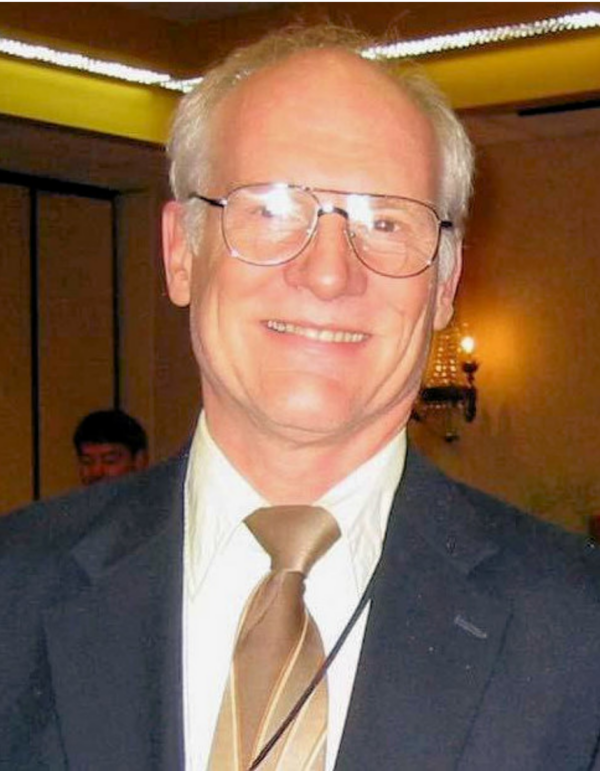
\includegraphics[width=0.25\textwidth]{./Chapter_1/bob_bruninga.png}
	\caption{Bob Bruninga.}
	\label{fig:bob-bruninga}
\end{figure}